\section{$L_1$因子分析}


\begin{frame}{$L_2$主成分分析不稳健}
    \begin{itemize}
        \item
        $L_2$主成分分析对离群值不稳健。
      \end{itemize}
    \begin{figure}[H]
        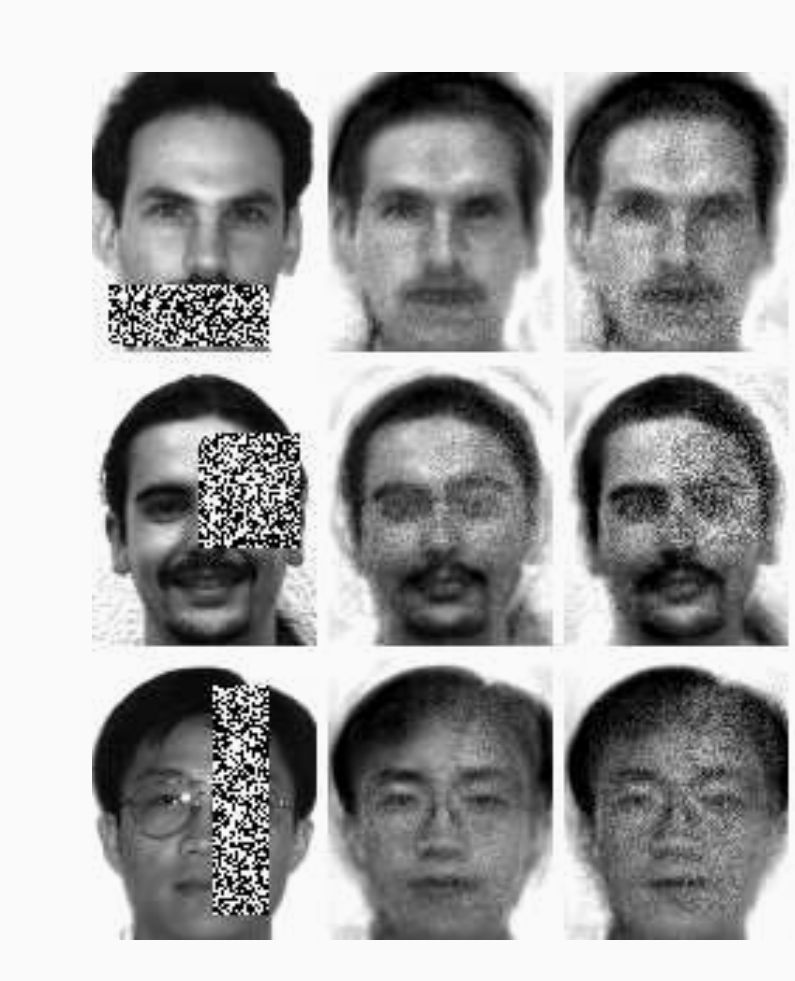
\includegraphics[width=5cm]{pics/face.png}
    \end{figure}
\end{frame}

\begin{frame}{
    $L_1$和$L_2$的稳健性对比}
    \begin{itemize}
        \item
        $L_1$范数能够提供更好的稳健性。
      \end{itemize}
    \begin{figure}[H]
        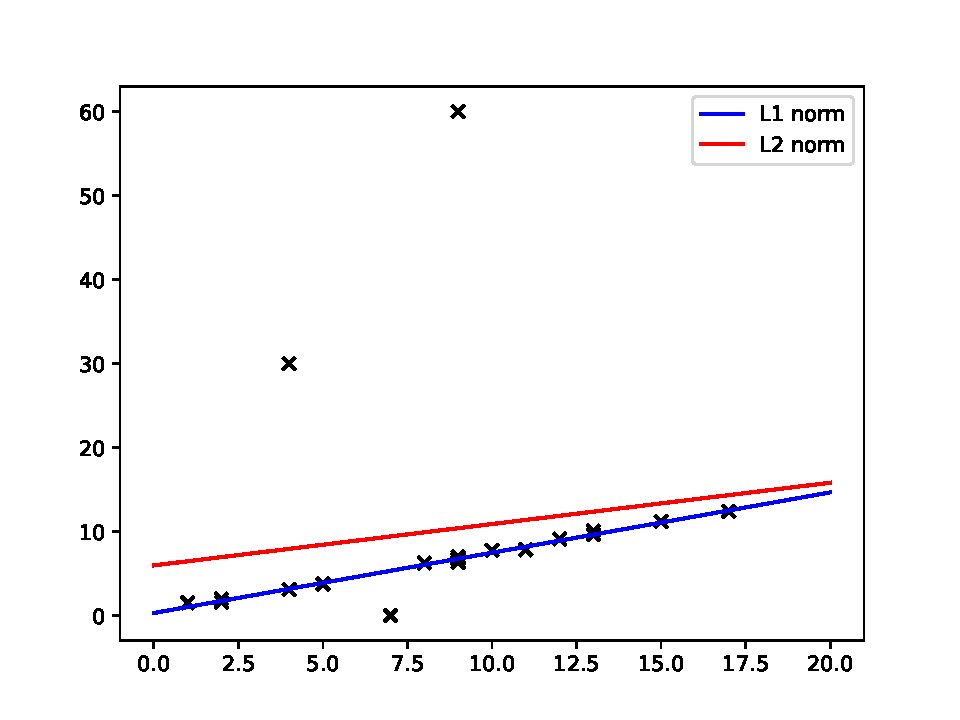
\includegraphics[width=5cm]{pics/l1-l2-diff.pdf}
        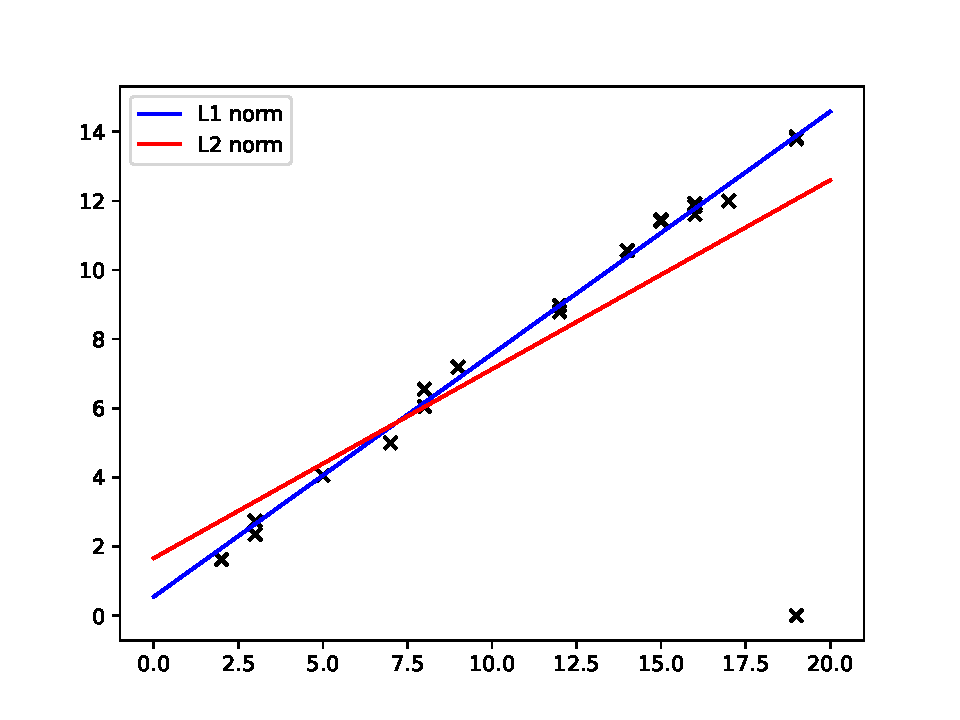
\includegraphics[width=5cm]{pics/l1-l2-diff2.pdf}
    \end{figure}
\end{frame}


\begin{frame}{$L_2$主成分分析问题描述}
    \begin{itemize}
        \item
        $L_2$主成分分析问题描述
    \end{itemize}
    \small
    \begin{equation}\label{pca-l2-p1}
        P_1: \ \hat{\bm{A}}_{p\times m}, \hat{\bm{F}}_{m\times n} = \underset{\bm{A},\bm{F}}{\operatorname{arg\ min} } 
        \|\bm{X} - \bm{A}\bm{F}\|_{L_2}
         = \underset{\bm{A}, \bm{F}}{\operatorname{arg\ min}} \sum_{i=1}^p \sum_{j=1}^m (x_{ij} - \bm a_i^T\bm f_i)^2 ,
        \end{equation}
    \tiny
        其中$\bm{X}$为$p \times n$的高维数据矩阵,$\bm{A}$的列构成了$\bm{X}$的$m$维线性子空间的基,这个子空间也称为特征空间。
        $\bm{F}$为一系数矩阵,给出了$\bm{X}$各列元素在特征空间中的坐标,根据矩阵投影理论,在给定$\bm{A}$的条件下,
        $\bm{F} = \bm{A}^T \bm{X}$。
        问题$P_1$可以解释为,需要找到一个合适的投射矩阵,使得数据在低维的投影上升回高维空间后和原矩阵各元素的误差平方和最小。
        
        对于问题$P_1$常用奇异值分解法求解。同样地我们也可考虑其对偶问题$P_2$,
    \small
        \begin{equation}\label{pca-l2-p2}
        P_2: \ \hat{\bm{A}} = \underset{\bm{A}}{\operatorname{arg\ max}} \| \bm{A}^T \bm{X}\|_{L_2}, \text{其中}\ \bm{A}^T
        \bm{A} = \bm{I}_m.
        \end{equation}
    \tiny
    问题$P_2$可以理解为,需要找到一个合适的投射矩阵,使得数据在低维空间的投影有最大的方差。在统计学上,数据的方差反映了
    数据中信息的多少,因此在特征空间中选取方差最大的方向作为主成分是很恰当的。
\end{frame}

\begin{frame}{重构误差最小化}
    \begin{figure}
        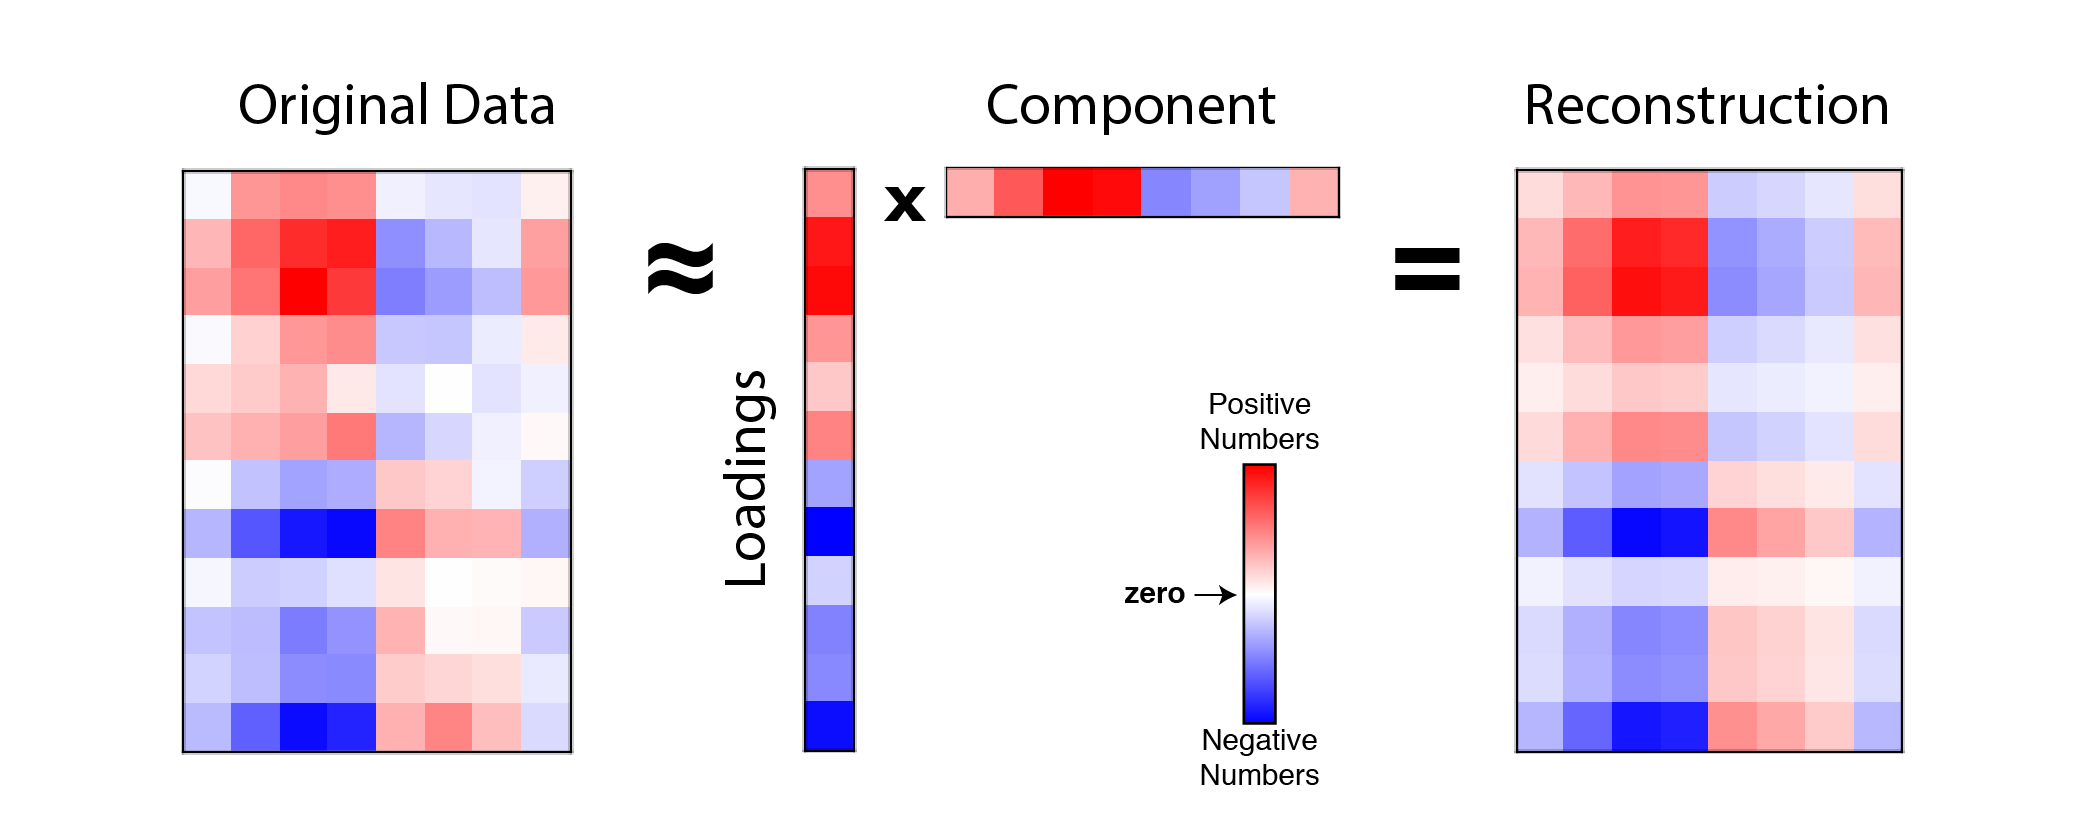
\includegraphics[width=10cm]{pics/recons-pcs.png}
    \end{figure}
\end{frame}

\begin{frame}{$L_1$主成分分析问题描述}
    \begin{itemize}
        \item
        $L_1$主成分分析问题描述
    \end{itemize}
    \small
    \begin{equation}\label{p3}
        P_3: \ 
    \hat{\bm{A}}_{p\times m}, \hat{\bm{F}}_{m\times n} = \underset{\bm{A},\bm{F}}{\operatorname{arg\ min} } \|\bm X - \bm{A}\bm{F}\|_{L_1}
    = \underset{\bm{A}, \bm{F}}{\operatorname{arg\ min}} \sum_{i=1}^p \sum_{j=1}^m |x_{ij} - \bm a_i^T \bm f_i|.
    \end{equation}
    \begin{equation}\label{p4}
        P_4: \ \hat{\bm A} = \underset{\bm{A}}{\operatorname{arg \ max}} \| \bm A^T \bm X\|_{L_1}
        = \underset{\bm A}{\operatorname{arg\ max}} 
        \sum_{i=1}^{n}\sum_{k=1}^{m}|\sum_{j=1}^p{a}_{jk}x_{ij}|
         \text{,其中}\bm A^T\bm A = \bm I_m
    \end{equation}
\end{frame}

\begin{frame}{一种$L_1$主成分分析的交替凸优化算法}
    \begin{itemize}
        \item
        Qifake \& Kande于2005年提出一种交替凸优化算法。
    \end{itemize} 
    \begin{table}[H]%%%%%%开始表格
        \tiny 
        \centering%把表居中
        \begin{tabular}{{p{0.9\columnwidth}}}%三个c代表该表一共三列,内容全部居中
        \toprule%第一道横线 表头
        交替凸优化求解$L_1$主成分分析 (ACP, Alternate Convex Programming) \\
        \midrule%第二道横线 符号+解释+单位 中间用&隔开
        1.初始化:给出$\bm{A}$,$\bm \Sigma$的初始值$\bm{A}^{(0)}$,$\bm \Sigma^{(0)} = \bm I$,(其中$\bm \Sigma$为一对角矩阵,
        $\bm I$为单位矩阵); \\
    
        2.交替凸优化:对于迭代次数$t = 1, ..., \tau$: \\
        $$ \bm F^{(t)} = \underset{\bm F}{\operatorname{arg\ min}} \|\bm X - \bm{A}^{(t-1)}\bm\Sigma^{(t-1)}\bm F^{T}\|_{L_1}$$ \\
        $$ \bm{A}^{(t)} = \underset{\bm{A}}{\operatorname{arg\ min}} \|\bm X - \bm{A}\bm\Sigma^{(t-1)}{(\bm F^{(t)})}^T \|_{L_1}$$ \\
        \begin{equation*}
            \text{归一化:}\left\{
                        \begin{array}{clr}
                        \bm N_a = diag({(\bm A^{(t)})}^T\bm{A}^{(t)})\\
                        \bm N_f = diag({(\bm F^{(t)})}^T\bm F^{(t)})\\
                        \bm F^{(t)} \leftarrow \bm F^{(t)}\bm N_f^{-1}\\
                        \bm{A}^{(t)}\leftarrow \bm{A}^{(t)}\bm N_a^{-1}\\
                        \bm \Sigma^{(t)} \leftarrow \bm N_a\bm \Sigma^{(t-1)}\bm N_f\\
                        \end{array}
            \right.
        \end{equation*} \\
    
        3.输出结果:$\bm{A} \leftarrow \bm{A}^{(\tau)}\bm \Sigma^{1/2}$,对$\bm{A}$进行QR分解取正交矩阵得到$\hat{\bm{A}}$;
        $\hat{\bm{F}} \leftarrow \hat{\bm{A}}^T\bm{X}$。 \\
        \bottomrule%第三道横线
        \end{tabular}
    \end{table}%%%%%%结束表格
\end{frame}

\begin{frame}{模拟实验准备}
    \begin{figure}[H]
        \centering
        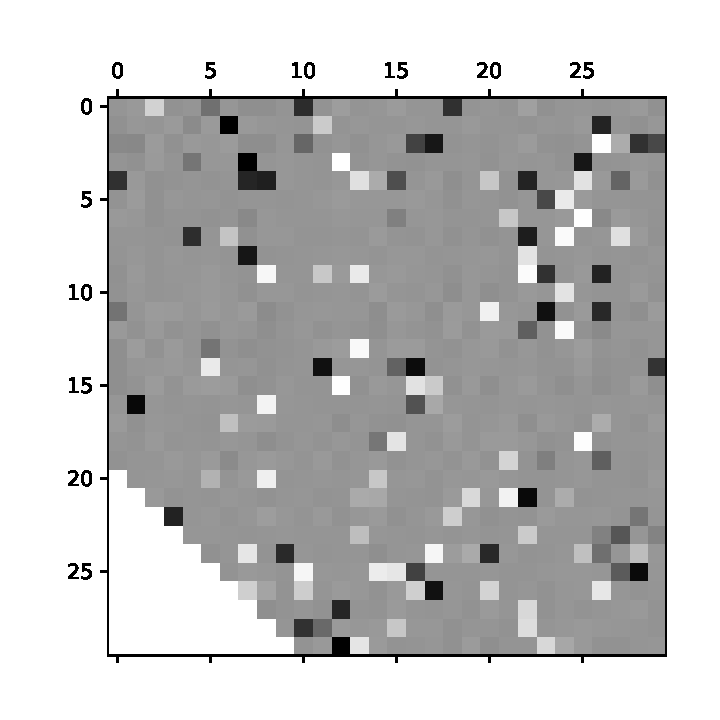
\includegraphics[width=.5\textwidth]{pics/matrix.pdf}
        \caption{\small $30\times30$的模拟矩阵}
        \label{fig2.1}
    \end{figure}
\end{frame}

\begin{frame}{模拟实验结果}
    \begin{figure}[H]
        \centering
        \begin{minipage}[t]{0.48\textwidth}
        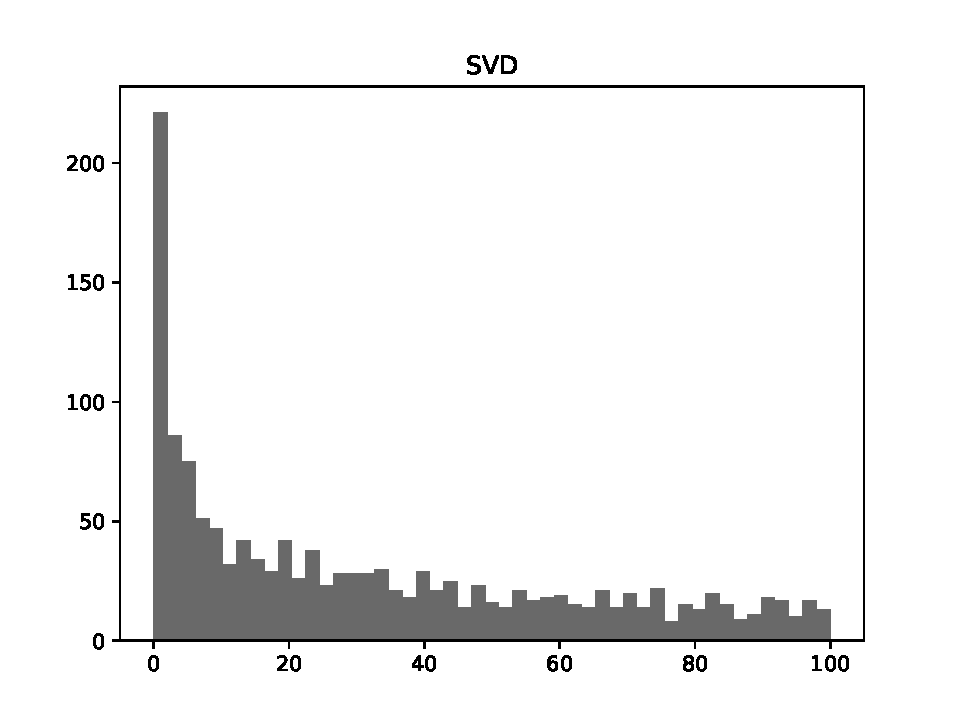
\includegraphics[width=5cm]{pics/svd.pdf}
        \end{minipage}
        \begin{minipage}[t]{0.48\textwidth}
        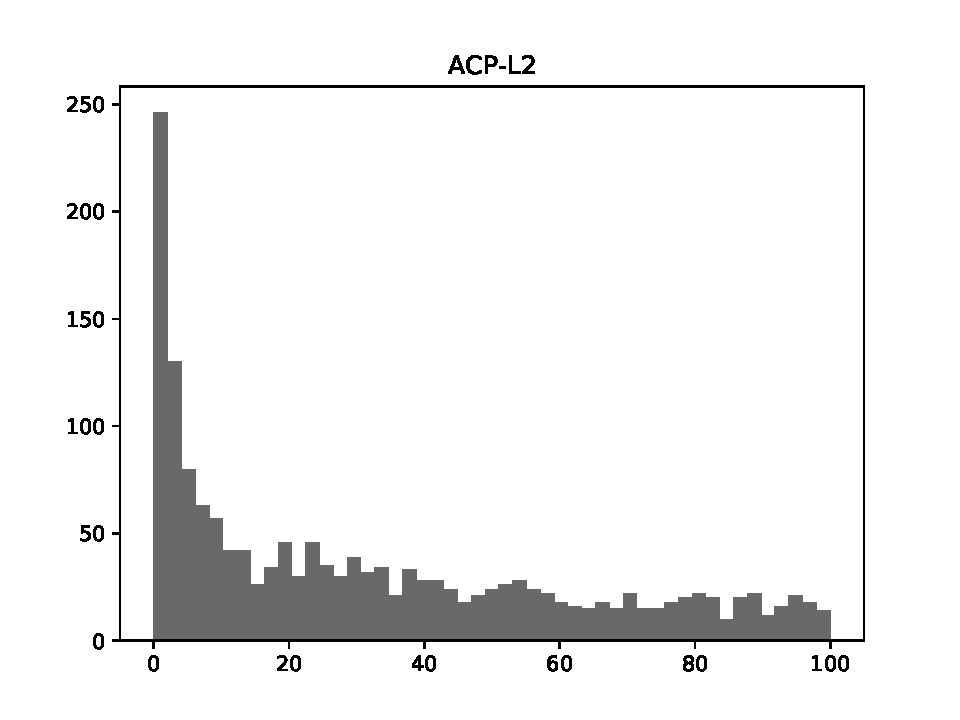
\includegraphics[width=5cm]{pics/acp-l2.pdf}
        \end{minipage}
        \begin{minipage}[t]{0.48\textwidth}
        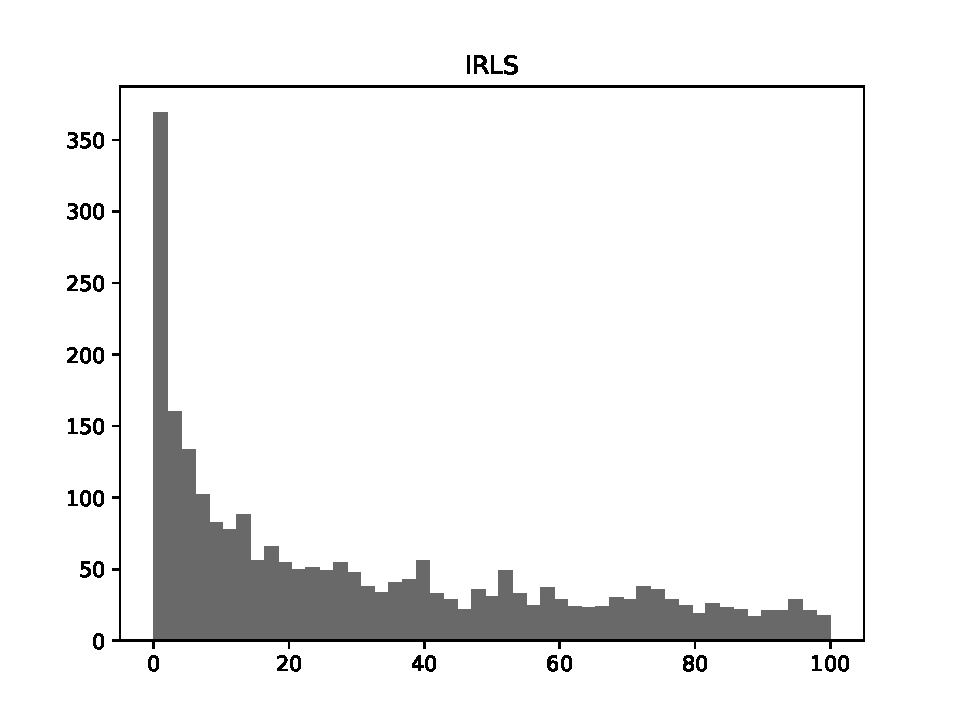
\includegraphics[width=5cm]{pics/IRLS.pdf}
        \end{minipage}
        \begin{minipage}[t]{0.48\textwidth}
        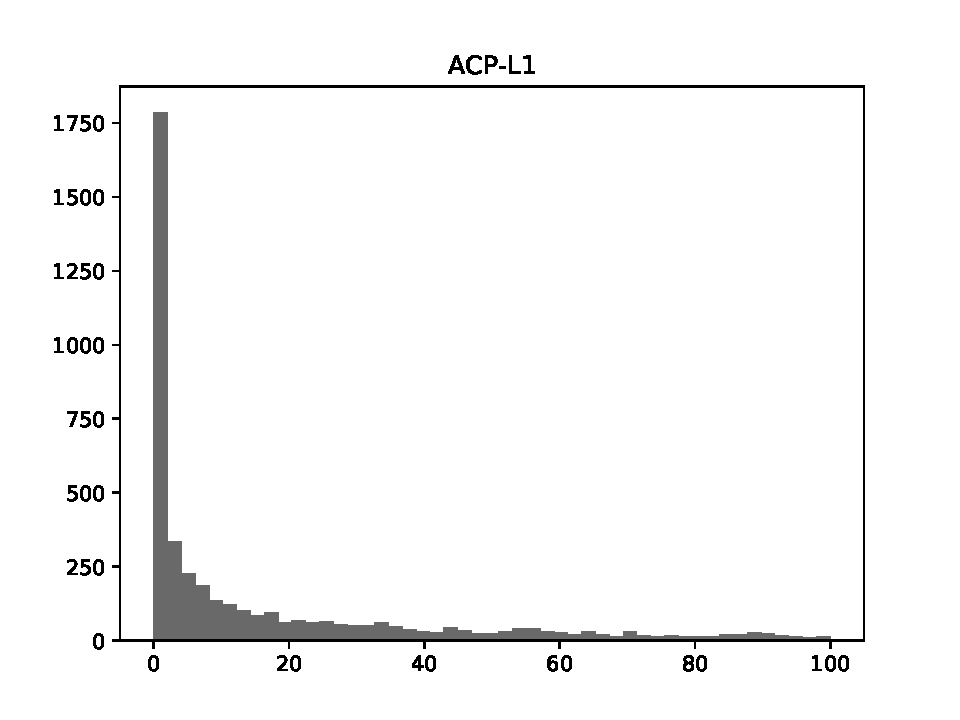
\includegraphics[width=5cm]{pics/acp-l1.pdf}
        \end{minipage}
    \end{figure}
\end{frame}

\begin{frame}{基于国内主要月度宏观经济数据的实证研究}
    \begin{itemize}
        \item
        数据来源:EPS数据平台-全国月度宏观经济数据
    \end{itemize}
    \begin{figure}[H]
        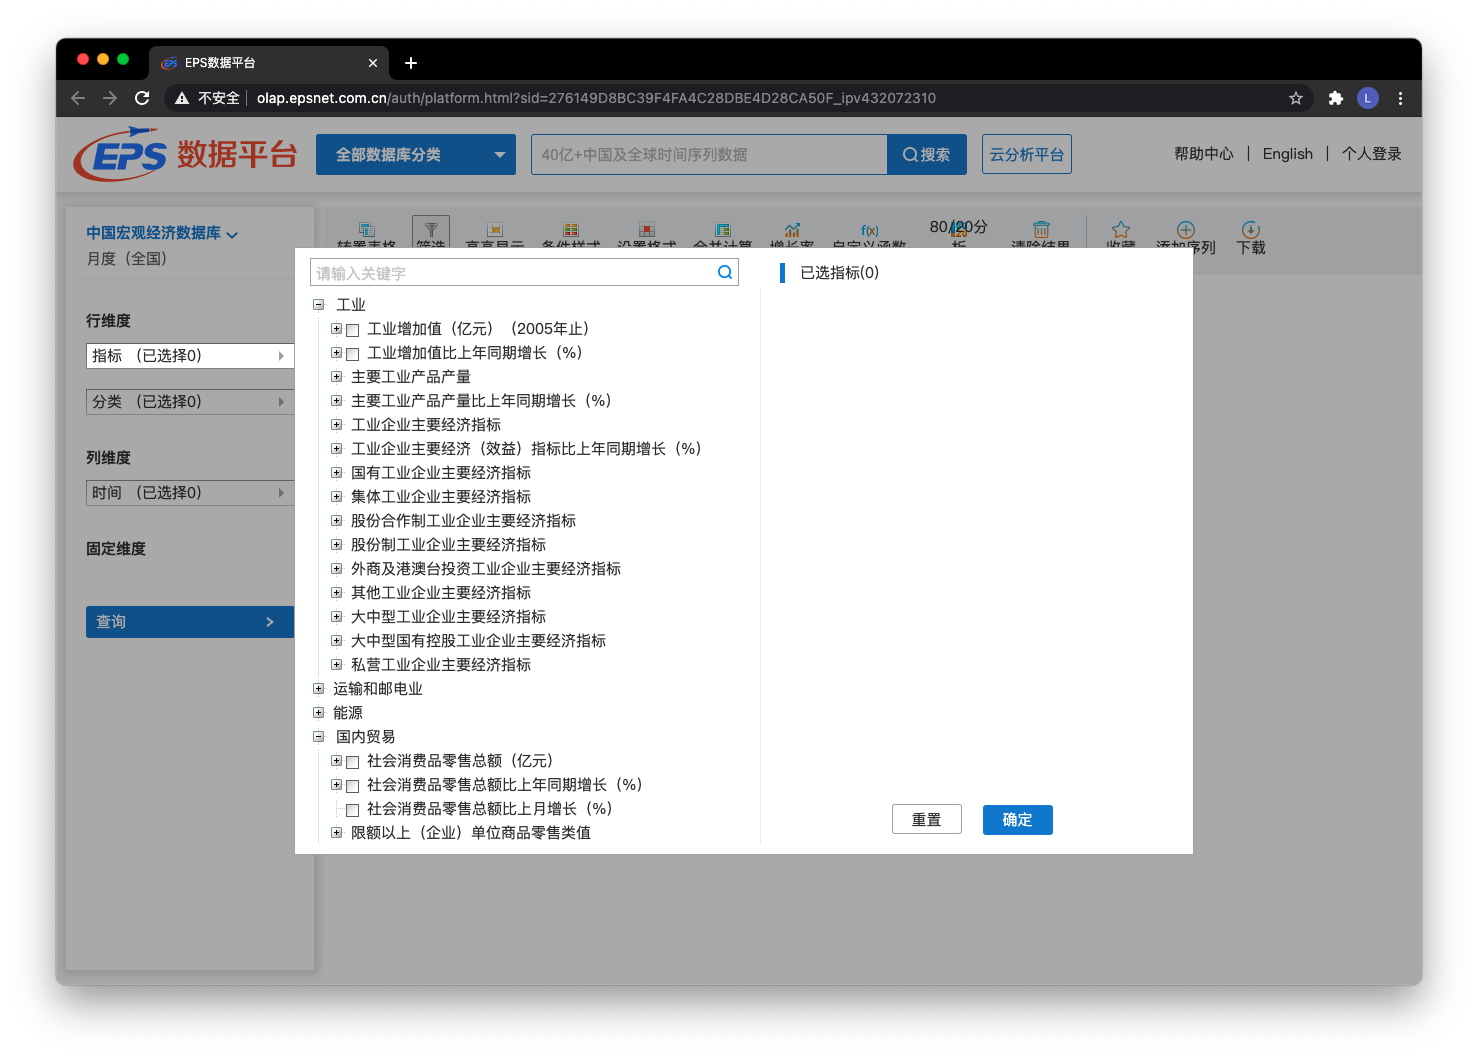
\includegraphics[width=9cm]{pics/data-source.png}
    \end{figure}
\end{frame}

\begin{frame}{基于国内主要月度宏观经济数据的实证研究}
    \begin{itemize}
        \item
        宏观经济数据的重尾性
    \end{itemize}
    \begin{figure}[H]
        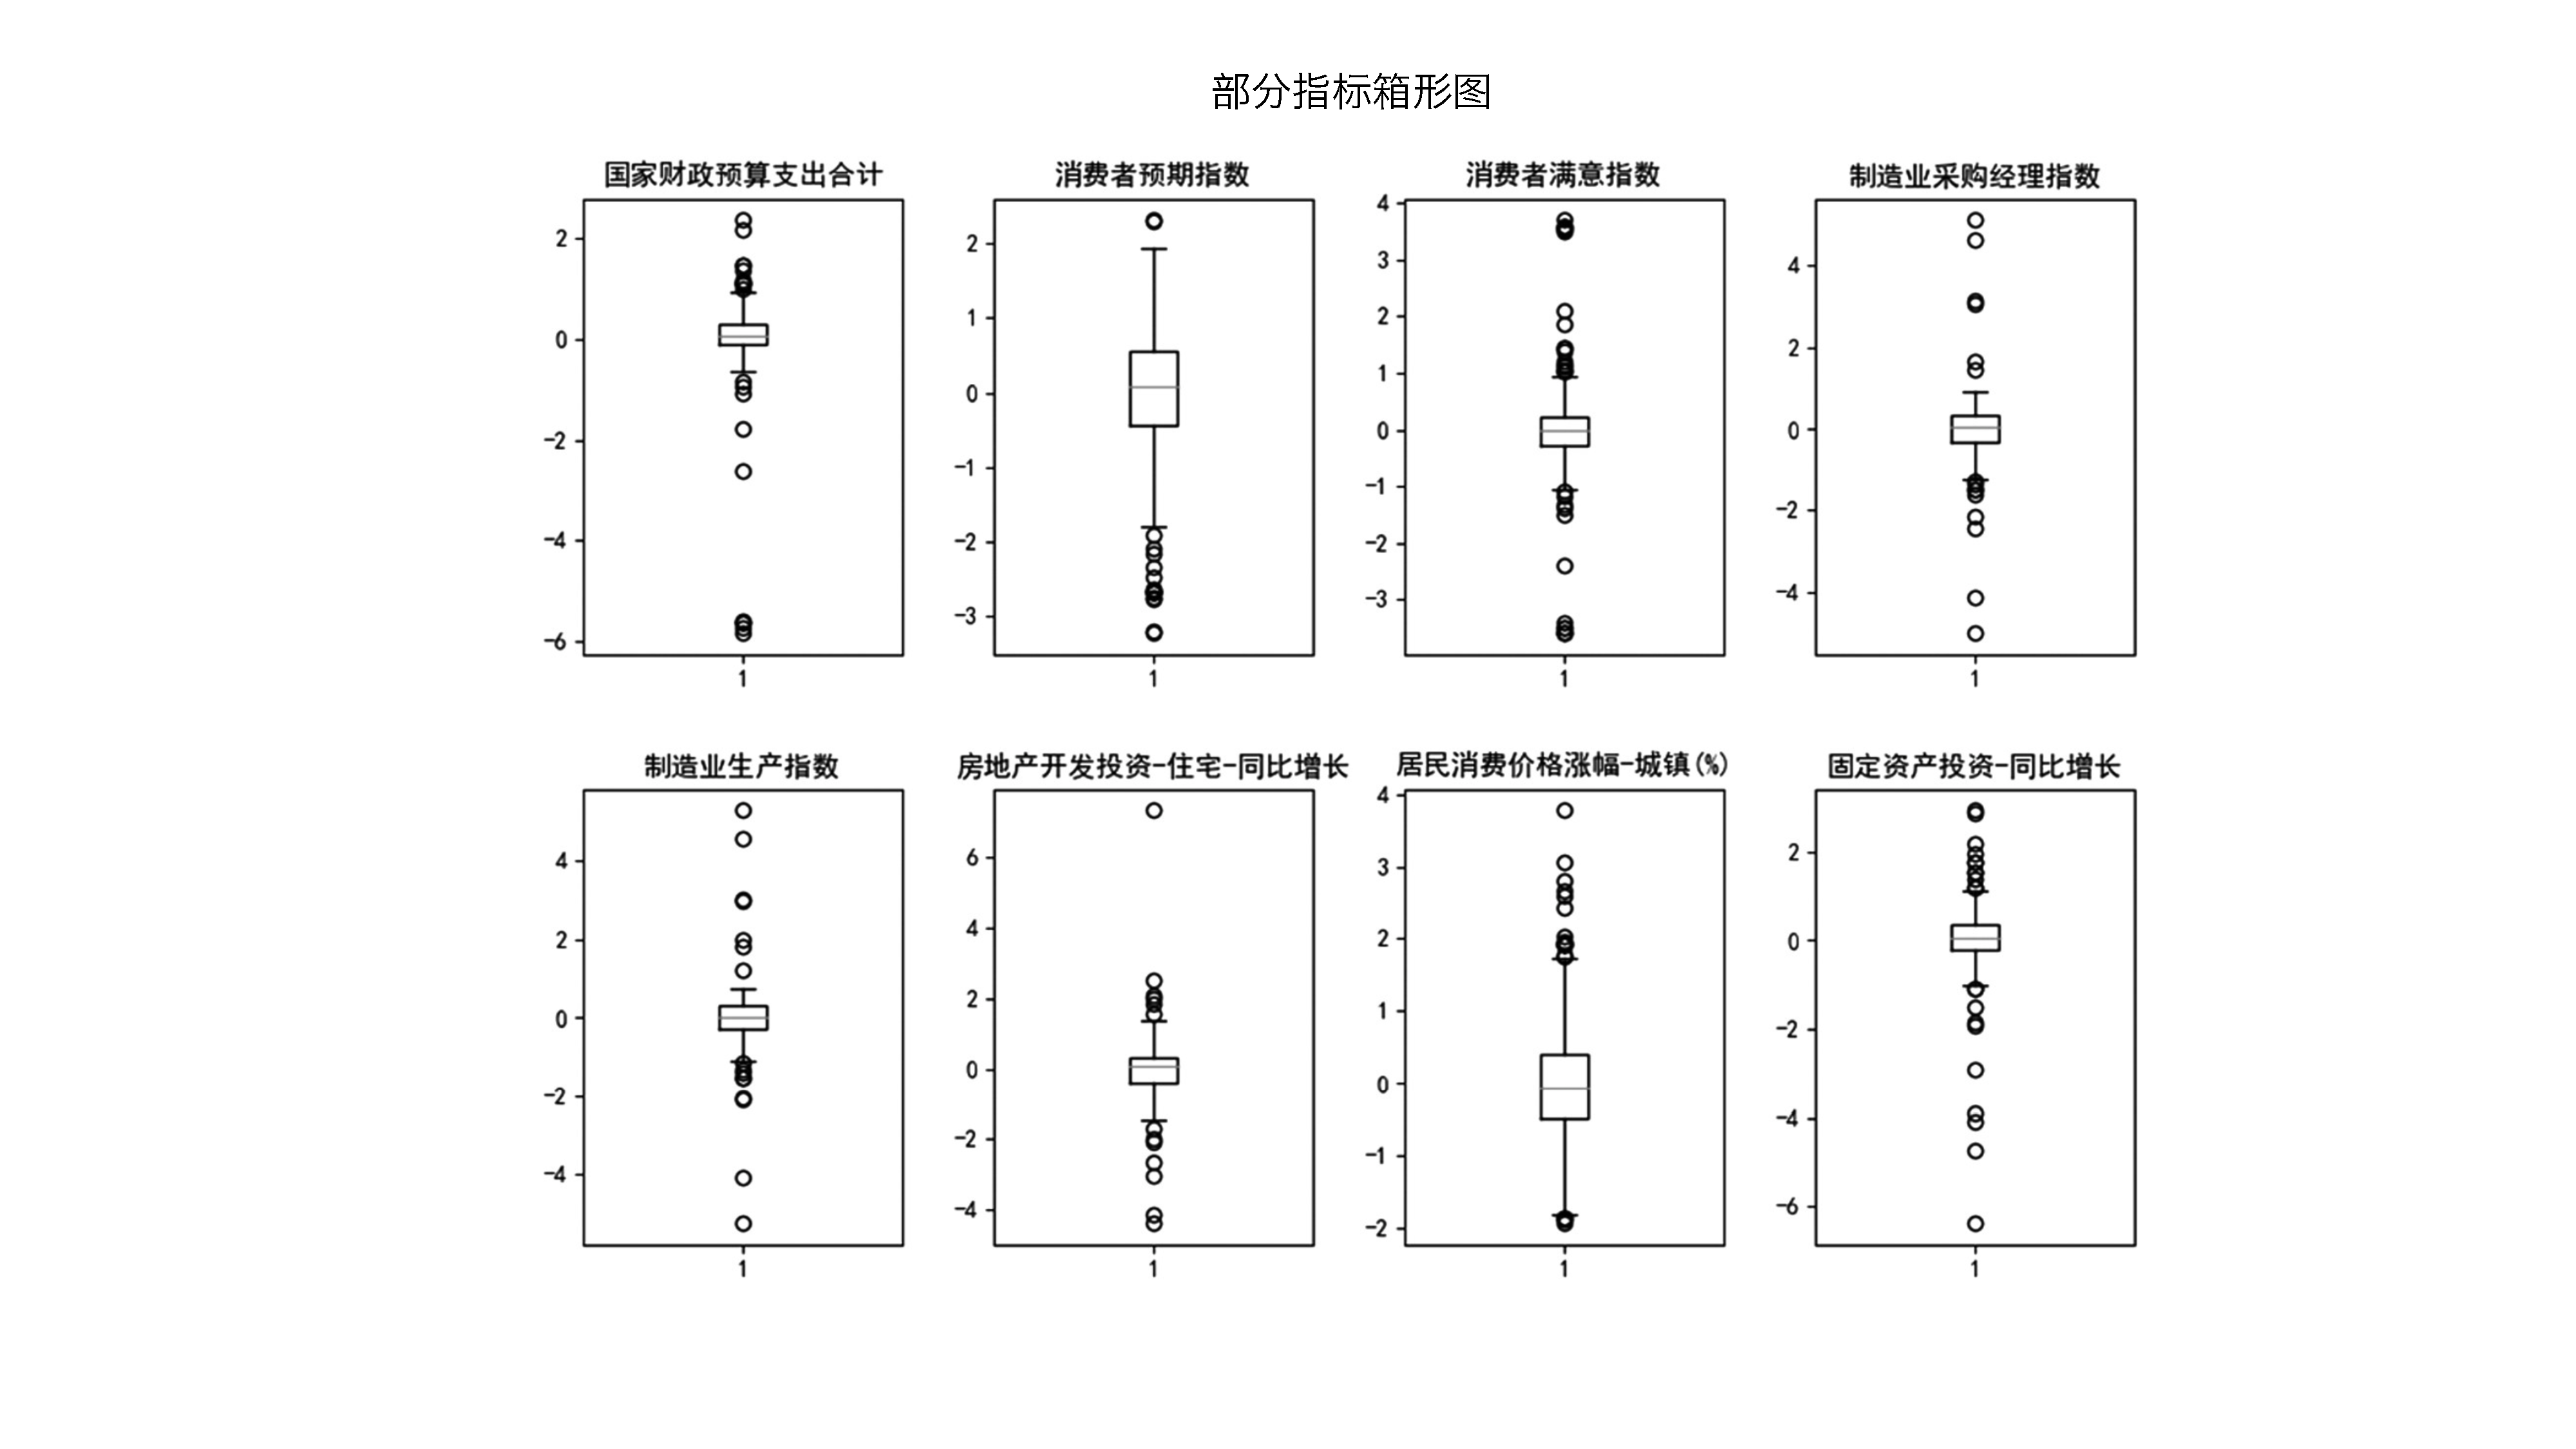
\includegraphics[width=10cm]{pics/box.pdf}
    \end{figure}
\end{frame}

\begin{frame}{基于国内主要月度宏观经济数据的实证研究}
    \begin{itemize}
        \item
        宏观经济数据的重尾性
    \end{itemize}
    \begin{figure}[H]
        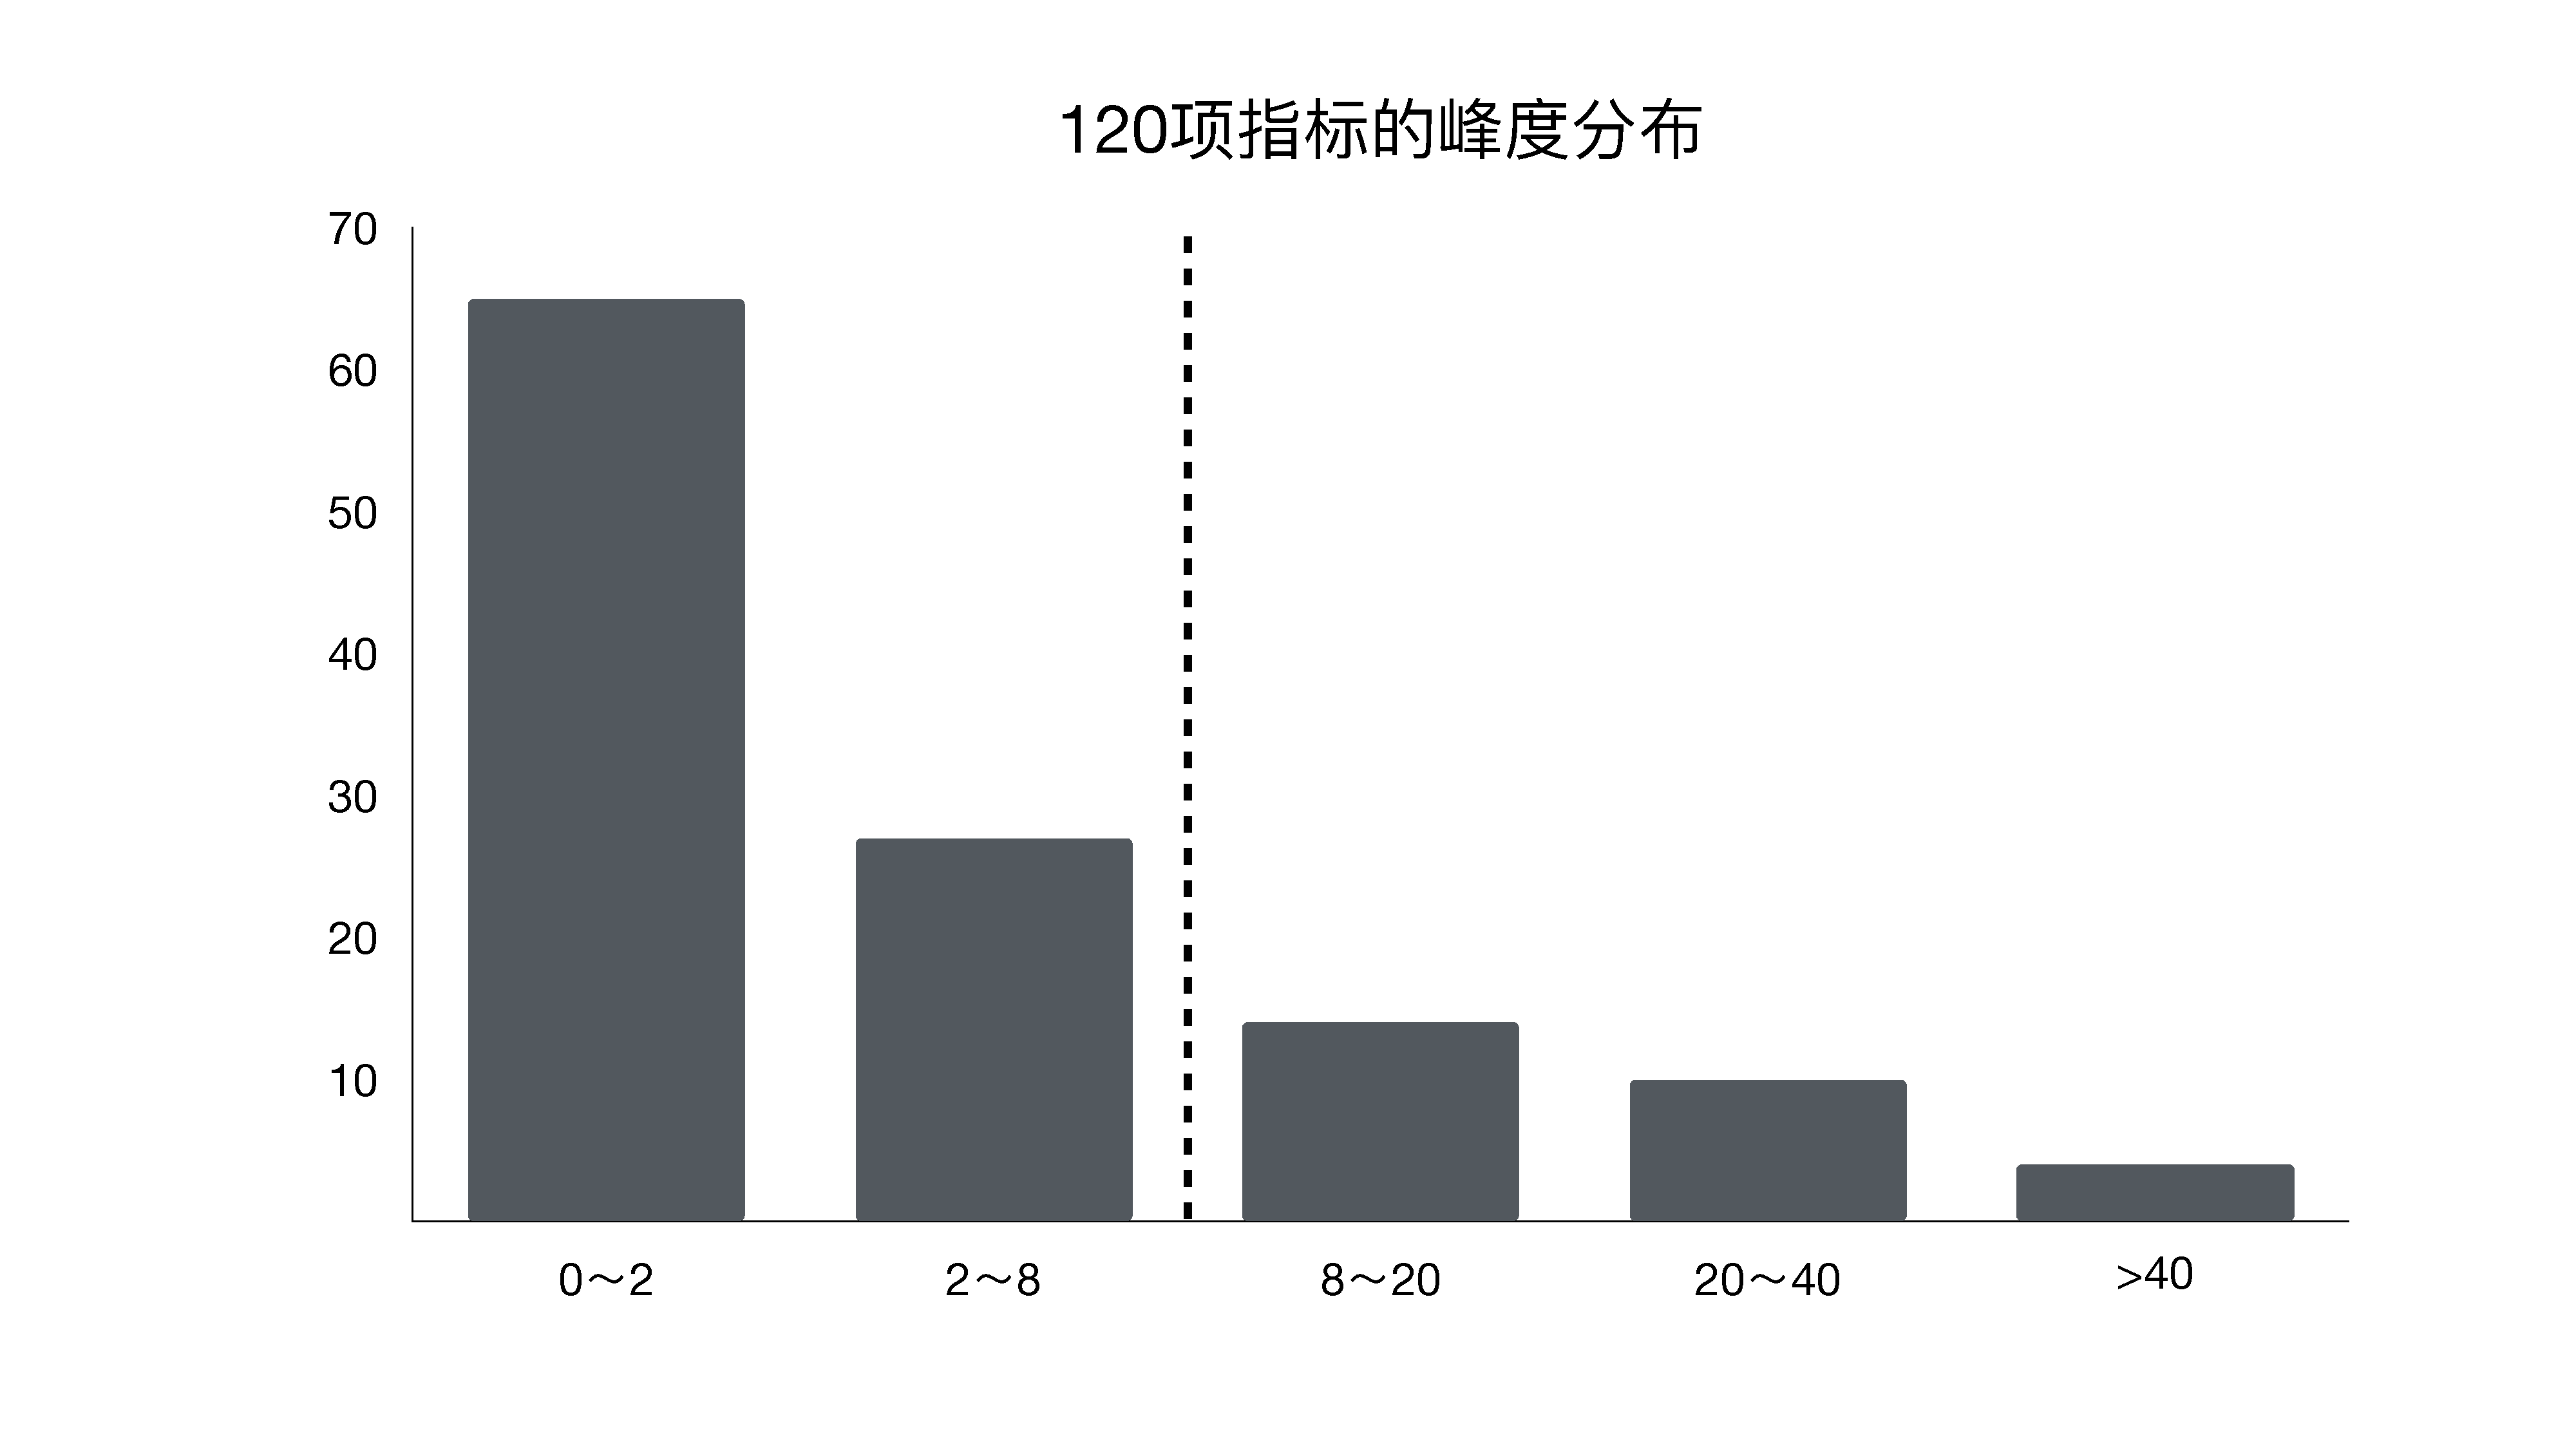
\includegraphics[width=10cm]{pics/skew.pdf}
    \end{figure}
\end{frame}

\begin{frame}{利用扩散指数模型进行预测}
    \begin{itemize}
        \item
        扩散指数模型预测
    \end{itemize}
\begin{equation}
    \bm{X}_t = \bm{A}\bm{F}_t + \bm{e}_t
\end{equation}
\begin{equation}\label{predict-factor-model}
    y_{t+h} = \bm{\beta}(L)\bm{F}_t + \bm{\alpha}(L)y_t + c + e_{t+h}
\end{equation}
\begin{itemize}
    \item
    因子个数选择,Bai\&Ng信息准则。
\end{itemize}
\end{frame}

\begin{frame}{利用扩散指数模型进行预测}
    \begin{itemize}
        \item
        滑动窗口预测
    \end{itemize}
    \begin{figure}[H]
        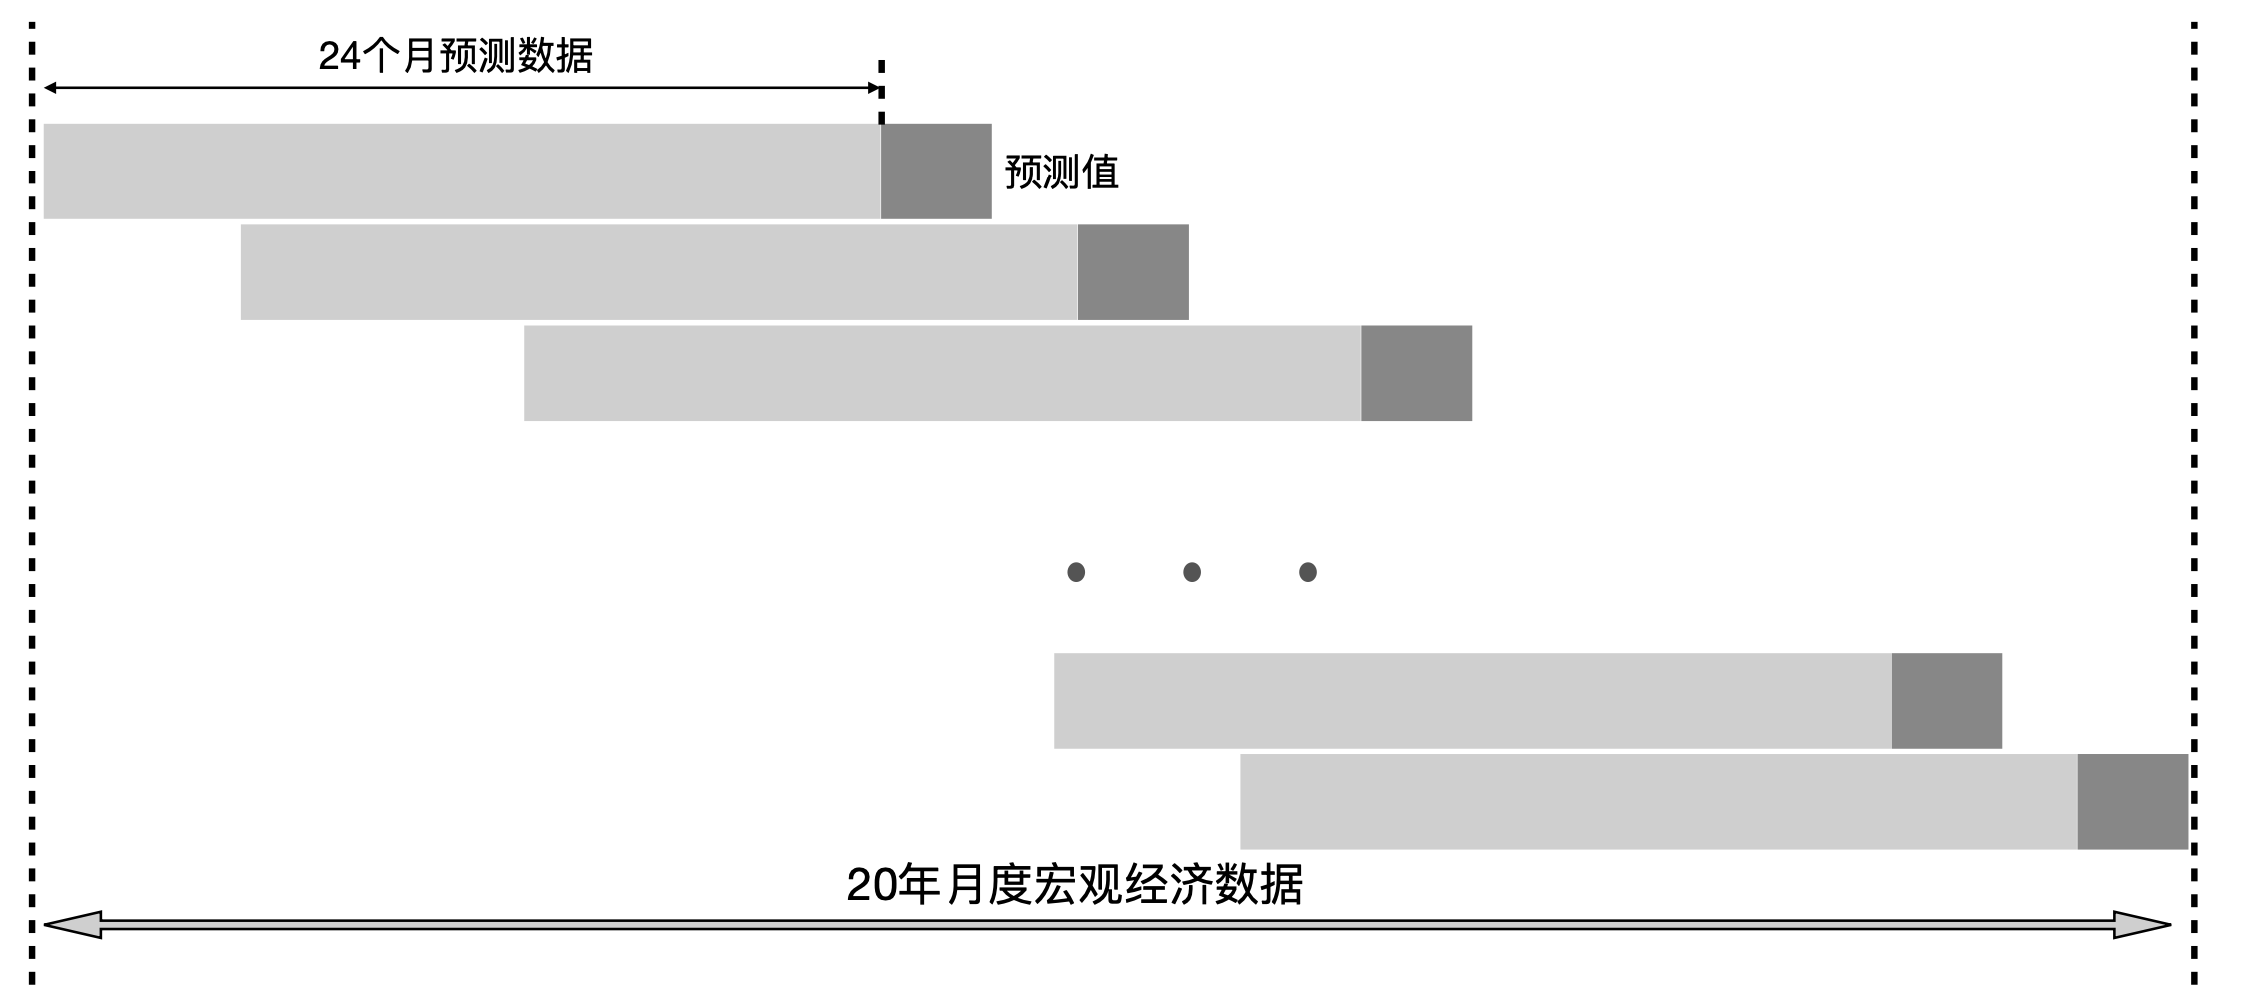
\includegraphics[width=10cm]{pics/predict.png}
    \end{figure}
\end{frame}

\begin{frame}{实证结果}
    \begin{itemize}
        \item
        预测结果表明:$L_1$因子在短期预测中比$L_2$因子更准确。
        长期预测,表现也良好。
    \end{itemize}
    \begin{table}[H]
        \tiny
        \caption{向前一个月预测结果}
        \label{outcome1}
        \centering
        \begin{tabularx}{\textwidth}{lXXXXXX}
        \toprule
                         &  MSE(L1 PCA) &  MSE(IM) &  MAE(L1 PCA) &  MAE(IM) &  MPAE(L1 PCA) &  MPAE(IM) \\ \midrule
        消费者满意指数*     & 0.81            & 1.49        & 0.87            & 1.67        & 0.43             & 1.55         \\
        工业生产者出厂价格指数* & 0.70            & 1.98        & 0.75            & 1.54        & 0.96             & 1.60         \\
        货币供应量M2*      & 0.76            & 1.25        & 0.90            & 1.19        & 0.45             & 0.97         \\
        固定资产投资总额*  & 0.89            & 1.03        & 0.97            & 0.99        & 0.81             & 1.32         \\
        房地产开发投资总额* & 0.79            & 0.98        & 0.95            & 1.00        & 0.91             & 1.20         \\
        社会消费品零售总额* & 0.84            & 1.25        & 0.87            & 1.12        & 0.45             & 1.17         \\
        制造业采购经理指数    & 1.24           & 1.69        & 1.06            & 1.43        & 0.90             & 1.50         \\
        住宅新开工面积总数*  & 0.89            & 2.40        & 0.85            & 1.98        & 0.45             & 2.22         \\
        股票流通市值*      & 0.99            & 3.99        & 0.98            & 2.84        & 0.81             & 4.51         \\
        消费者信心指数*     & 0.93            & 1.01        & 0.98            & 0.99        & 0.98             & 1.56         \\ \bottomrule
        \end{tabularx}
    \end{table}
\end{frame}